\documentclass[conference]{IEEEtran}
\IEEEoverridecommandlockouts
% The preceding line is only needed to identify funding in the first footnote. If that is unneeded, please comment it out.
\usepackage{cite}
\usepackage{amsmath,amssymb,amsfonts}
\usepackage{graphicx}
\usepackage{textcomp}
\usepackage{xcolor}
\def\BibTeX{{\rm B\kern-.05em{\sc i\kern-.025em b}\kern-.08em
    T\kern-.1667em\lower.7ex\hbox{E}\kern-.125emX}}
\begin{document}

\title{CENG 435 NETWORK AND COMMUNICATION SYSTEMS TERM PROJECT PART-1 REPORT \\
{\footnotesize}
\thanks{}
}

\author{\IEEEauthorblockN{ Mustafa BADILLI}
\IEEEauthorblockA{\textit{2171296} \\
\textit{Group-63}
}
\and
\IEEEauthorblockN{ Sahin KASAP}
\IEEEauthorblockA{\textit{2264562} \\
\textit{Group-63}
}
}

\maketitle

\section{Overview}
\subsection{General Look}
In this project, it was expected to construct a network with 5 nodes named s (for source), r1,r2,r3(routers) , and d(for destination). These nodes are connected to each other (r1 and r3, s and d are not connected but all of the others are). This part of the project consists of implementing a UDP (User Datagram Protocol), and testing our environment using this protocol. The aim of the experiment is to find the cost of the links, using network emulator and finding the best route on different environments. 

\subsection{Concerns About Design}
We first of all need to care about our design. Firstly we need to construct protocols between nodes. After constructing the protocols, we need to choose what to share between nodes. The main aim of the experiment is to find the delay time between nodes, so we have save the time the packet is sent and the time the packet is received. And we must find the best route, so we need to care about the roads. One of the most important things that we had difficulties about was to find out the IP address and port numbers to write. The IP and the port numbers in the programs of client and the server must be the same. Python allows us both in TCP and UDP but as we required to do the assignment in UDP, we used socket library such that we connected client and server in UDP. 

\subsection{How To Carry Out The Program}
We chose Python programming language for the experiment for its easiness and simplicity. We imported time library to measure proper time delays between nodes; socket library in order to have a connection between nodes over network, and Thread library in order to have a proper working program. In order to be using UDP, we used socket with AF\_INET and SOCK\_DGRAM, AF\_INET is used to specify the program's address family. We can use addresses of type AF\_INET with the socket. And SOCK\_DGRAM means its protocol is UDP (User Datagram Protocol). After creating sockets and writing their IP and ports properly, we can start the program. It is better to start the destination first, because it listens and gives feedback. Without it listening, even though we start the other programs, they will not get an answer to their sent messages. After starting all programs (clients and servers), we can see the files are getting sent. The time measurements must be kept in a file. After the execution of programs, the average times that are kept in measurements file is observed and the best route is found using Dijkstra algorithm. 

\section{Procedure}
In this project, r1 and r3 are always clients. S and D are always servers and r2 is client and server at the same time. S and D always listen to the connection and they don't stop without us stopping them. Clients send 1000 words, one word each time, and waits for receiving some response and saves the time. After all of the files sent, the average time is taken, this time gives us some information about the speed of the road. After finding speeds of all roads, we can find the fastest way from S to D. \\
The results is shown below:\\
r1 to S  : 0.61683\\
r1 to r2 : 0.141583\\
r1 to D  : 0.61670\\
r2 to S  : 0.081458\\
r2 to D  : 0.814626\\
r3 to S  : 0.00105780\\
r3 to r2 : 0.0817653\\
r3 to D  : 0.00105907\\
If we apply Dijkstra Algorithm, we find that the best way from S to D is S-r3-D
\section{Motivation}
This project helped a lot about learning network systems and protocols. We connected two devices together and send/receive information. This was so pleasing. This was a great step to learn network and connections. There are a lot more than that, and we are willing to learn more.
\section{Experimental Results}
In experiment part, we used netem to delay the sendings of the packets. We repeated the sending of packets 100 times to get a good result. And we averaged the total delay. We used normal distribution.
\begin{figure}
    \centering
    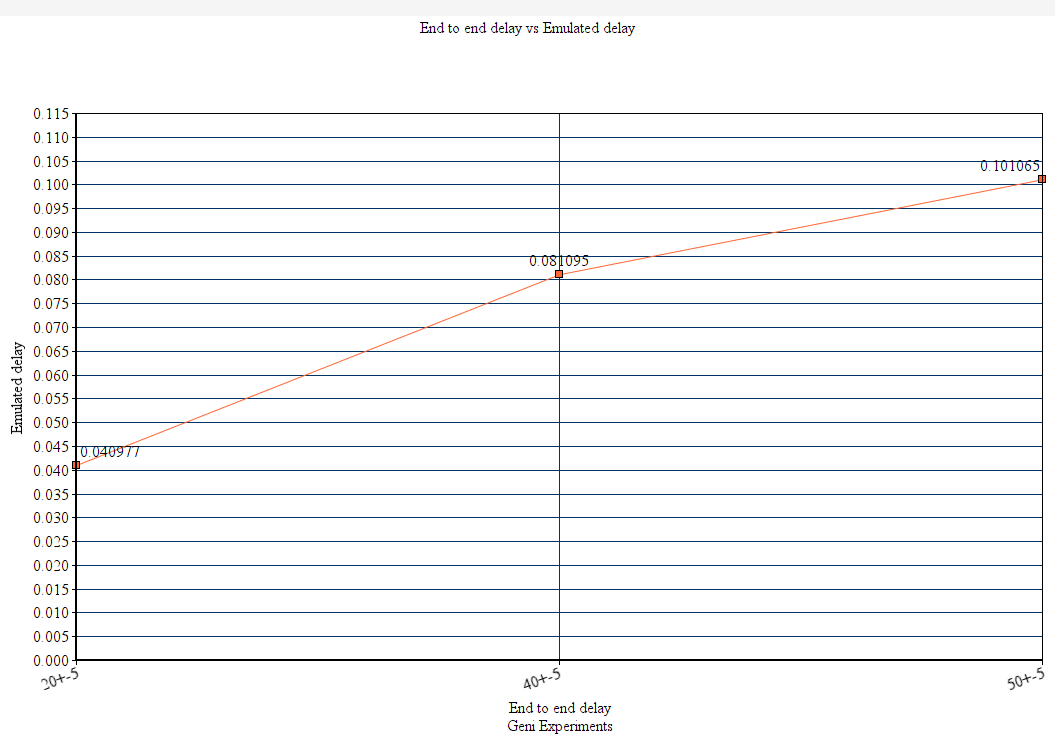
\includegraphics[scale=0.62]{Delaysandresults.png}
    \caption{Average delay with Netem}
\end{figure}

Shown in the figure, the 20 +- 5 ms delays caused 0.040977 second delays. 40+-5 ms delays caused a 0.081095 second delays and 50 +- 5 ms delays caused 0.101065 second delays. These are expected results, since we delay both sides of the connection the results are nearly two times of the delay time we give. The delay doesn't seem to effect other things. The network emulator can be used in many things, we can simulate a router without having a router and see the results, the best way to send a packet etc.\\
If we try to calculate if delaying effected the program other than just delaying, we can look at the older results. R3 to S and getting back was 0.00105780 s, R3 to D and getting back was 0.00105907 s. If divide them to two and sum we get 0,001058435 s. 20 ms delay for both sides makes 40 ms. If we sum them up, we get 0.041058435. There doesn't seem to be any difference. \\
In order to 

\section{What We Understand From The Project}

In this project, we learned the general structure of network systems and protocols. I think this was a really good experiment and project. We learnt lots of things in the lessons and by this project we truly understand the network and protocol. We now, actually can have a connection between two computers with a little bit knowledge to connect devices together. 

\end{document}

